%!TEX encoding = UTF-8 Unicode
\documentclass[letterpaper,11pt,english,twocolumn]{article}

\usepackage[T1]{fontenc}
\usepackage[utf8]{inputenc}
\usepackage{babel}
\usepackage{indentfirst}
\usepackage{cite}
\usepackage[colorlinks]{hyperref}
\usepackage{graphicx}
\usepackage{paralist}
\usepackage{amsmath,amssymb}
\usepackage{footnote}
\usepackage[binary-units=true]{siunitx}
\usepackage[inline]{enumitem}

\usepackage[calc,style=default]{datetime2}
\DTMsetup{datesep={--},datetimesep=T}


\title{
	\begin{center}
  		
\includegraphics[width=0.125\textwidth]{./images/units-logo.pdf}\\
  		\smallskip
  		\Large {University of Trieste}\\
		\smallskip
  		\large \textit{Introduction to Machine Learning} Course\\
		\smallskip
		\small Academic Year 2022--2023\\
  		\rule{9cm}{.4pt}\\
		\medskip
  	\end{center}
	Predicting the popularity of food tweets
}

\author{
	Enrico Stefanel [SM3500554]\thanks{Data Science and Scientific Computing Master's student, \href{mailto:enrico.stefanel@studenti.units.it}{\texttt{enrico.stefanel@studenti.units.it}}}
}


\DTMsavenow{now}%
\DTMtozulu{now}{currzulu}
\date{\footnotesize Last update on \DTMuse{currzulu}.}
%\date{\today}

\begin{document}

\maketitle

\begin{abstract}
We compare different Machine Learning models that use Text Mining techniques to estimate how popular would a tweet containing the word \textit{food} be, if published on Twitter. In particular, we study application of linear regressors, Decision trees and Random forests to find the best model in terms of MSE and prediction times.

After a little introduction to the problem statement and some preliminary analysis in \autoref{sec:problem_statement}, we describe assessments index that are used to compare different models in \autoref{sec:assessment_performance_indexes}. Next, in \autoref{sec:solution} we describe the proposed solution, and the experimental methods in \autoref{sec:experimental_evaluation}. Finally, we draw conclusions and come up with possible future improvements in \autoref{sec:conclusions}.
\end{abstract}


\section{Problem statement}
\label{sec:problem_statement}
We are required to build a tool for predicting \textit{how popular} will be a tweet about food.
We are not provided with a dataset, and we are requested to autonomously obtain it.

Formally, given the sets $X$ and $Y$ defined as
\begin{align*}
\begin{gathered}
	X = \{x \mid x \text{ is a tweet}\}\\
	Y = \mathbb{R},
\end{gathered}
\end{align*}

our goal is to learn a model $m \in M$ from the function $f'_{learn}$ and use it to predict the response variable using a $f'_{predict}$, where the two functions are defined as
\begin{align*}
\begin{gathered}
	f'_{learn}: P^{*}(X \times Y) \rightarrow M\\
	f'_{predict} : X \times M \rightarrow Y.
\end{gathered}
\end{align*}

A solution based on Machine Learning is suitable for the proposed problem: building a $f_{learn}$ function can not be done by humans, because of human costs and solution complexity (we are dealing with tens of thousands of observations, each with hundreds of features). We expect the model $M$ to be not very simple, so also running $f'_{predict}$ on a machine is the only way.

Given the nature of $X$ and $Y$, we can (and indeed will) use supervised learning techniques for our purposes.


\section{Assessment and performance indexes}
\label{sec:assessment_performance_indexes}
Recalling that the response variable $Y$ we are dealing with is numeric and continuous, it is natural for us to think of using Mean Squared Error (MSE) for measuring models \textit{effectivness}.
As for the \textit{efficiency} of the solutions, we focus on the prediction times rather than the learning ones, since this last are transparent to the final users. We are going to measure the time taken by the model to predict all the response variables $y^{(i)}$ in the test set by repeating the prediction for $1000$ times and taking the mean of total time.
We are also keeping in consideration that a model that uses a lower number of features for the estimation of the response variable is more \textit{interpretable} by humans than a more complex one.

\section{Proposed solution}
\label{sec:solution}
After retrieval of the dataset, a total of four different learning techniques have been tested for the prediction:
\begin{enumerate*}[label=(\roman*)]
	\item Dummy regressor,
	\item Linear models,
	\item Regression trees and
	\item Random Forests.
\end{enumerate*}
For some of these families (those that are particularly promising), we deepened the study by trying to optimise learning parameters.
At the end, we compared models by \textit{effectiveness} and \textit{efficiency}.


\section{Experimental evaluation}
\label{sec:experimental_evaluation}
The whole project is implemented using the $R$ programming language, and all the code is publicly available at \url{https://github.com/enstit/TweetPopularityPrediction}.

\subsection{Data retrieval}
\label{ssec:dataretrieval}
We are not going into details about how we collected the data, because it is not this project purpose.
To summarise, we used Twitter APIs \cite{DBLP:journals/corr/abs-2105-10724} to collect a set of $50000$ tweets containing the word ``\textit{food}'', written in english and published during the 2022 Christmas day (in CET time). Each observation includes the tweet text and date-time, tweet metrics (likes, retweets, replies), user metrics (following, followers) as well as media informations for those tweets that also include an image, video, or animated gif, plus other features that has not been used in the study because they clearly are not influential (e.g., the tweet author full name and username). This leads to a total of twenty-two columns for each observation.

As regarding the response variable, we know that the popularity of a tweet is surely correlated with the number of likes, retweets and replies to that. But, on the other hand, we also \textit{expect} this insights to be high for a tweet published by a user with many followers. To take this into consideration, we divide the sum by the number of user followers. We then increase both numerator and denominator by one, to ensure that a finite index exists, and take the natural logarithm.
\begin{align*}
\begin{gathered}
	y^{(i)} = \ln \left( \frac{1+x^{(i)}_{likes}+x^{(i)}_{retweets}+x^{(i)}_{replies}}{1+x^{(i)}_{followers}} \right)
\end{gathered}
\end{align*}

\subsection{Procedure}
\label{ssec:procedure}
After reducing the dataset to the tweet text and the attached media type feature, we performed text pre-processing on the tweets corpus (lowercase conversion, punctuation and numbers removal, stemming, stop-words removal). To vectorise documents tests, we used a TF-IDF function \cite{DBLP:journals/corr/abs-1901-09069} and only kept terms that appeared in at least $1\%$ of the documents.

The final dataset counts of $202$ features and a response variable.

We then divided the dataset into static training and test dataset, with a $80:20$ proportion. We decided to do not use \textit{cross validation} since the dataset is big enough and evenly distributed (as shown in figure \autoref{fig:image}), thus the effective improvements would not be significant to justify degradation in learing-phase efficiency.

\begin{figure}
    \centering
    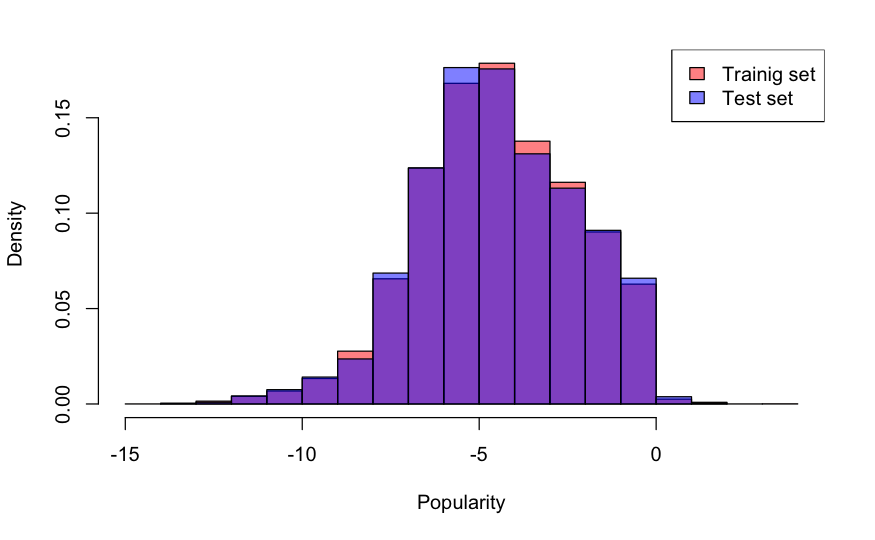
\includegraphics[width=.5\textwidth]{./images/hist.png}
    \caption{Distribution of \textit{popularity index} in training and test sets.}
    \label{fig:image}
\end{figure}

All models have been trained on the training set, and evaluated on the test set.

\subsubsection{Dummy regressor}
The Dummy regressor, used as a baseline to assess all the other most evolved models, is the one that always predict the mean value of $\{y^{(i)}\}_i$.
\begin{align*}
\begin{gathered}
	f_{dummy,\{y^{(i)}\}_i} (x) = \frac{1}{|y|} \sum_{i=1}^{|y|} y^{(i)} 
\end{gathered}
\end{align*}


\subsubsection{Linear model}
After learning a complete linear model using all the 202 features, we also tried, using a \textit{step-wise algorithm} procedure \cite{10.48550/ARXIV.1605.01936}, to reduce the number of that (so that the model \textit{interpretability} increases) only keeping those who are justified by a dropping in AIC index if retained. This model ended by having about $60\%$ of the original predictors ($118$ versus $205$), but scoring a very similar MSE on the test set (even slightly lower) and being about $40\%$ faster on predictions.

\subsubsection{Regression tree}
The model we tested next has been the Regression tree.
Compared with the default values of $R$ function \texttt{rpart} \cite{rpart}, only the complexity parameter \texttt{cp} has been lowered from $0.01$ to $0.0001$. This led the model to use $189$ predictors (compared with only $13$ if we left \texttt{cp} to its default value).


\subsubsection{Random forest}
Finally, a Random forest model has been trained. At the beginning, we trained the model using the default values of the \texttt{randomForest} function in $R$ \cite{randomForest}. Then, we decided to slim down the model reducing the number of trees from $500$ to $250$ and lastly to $100$. Having obtained satisfactory results with the latter option, we also proceeded to increase the minimum number of observations in leaf nodes from $5$ (default value) to $50$ and then to $100$ to make the model even simpler (and thus faster in predictions).


\begin{table}%[h!]
\centering
 \begin{tabular}{||l r r||} 
 \hline
 \multicolumn{1}{||c}{Model} & \multicolumn{1}{c}{MSE} & \multicolumn{1}{c||}{$\mu_{p.time}$} \\
 \hline\hline
 Dummy regressor & 5.216 & 0.400 \\
 Linear model & & \\
 \quad \rotatebox[origin=c]{180}{$\Lsh$} $n_{var}=118 \ll p$  & 4.137 & \textbf{11.048} \\
 \quad \rotatebox[origin=c]{180}{$\Lsh$} \underline{$n_{var}=205=p$} & 4.138 & 18.267 \\
 Regression tree & 3.947 & 25.502 \\
 Random forest & &  \\
 \quad \rotatebox[origin=c]{180}{$\Lsh$} $n_{tree}=100$ & & \\
 \qquad \rotatebox[origin=c]{180}{$\Lsh$} $n_{min}=100$ & 3.746 & 396.545 \\
 \qquad \rotatebox[origin=c]{180}{$\Lsh$} $n_{min}=50$ & \textbf{3.741} & 465.842 \\
 \qquad \rotatebox[origin=c]{180}{$\Lsh$} \underline{$n_{min}=5$} & 3.765 & 718.422 \\
 \quad \rotatebox[origin=c]{180}{$\Lsh$} $n_{tree}=250$ & 3.748 & 1705.838 \\
 \quad \rotatebox[origin=c]{180}{$\Lsh$} \underline{$n_{tree}=500$} & 3.747 & 3295.462 \\
 \hline
 \end{tabular}
 \caption{Models MSE and prediction times (in milliseconds) measured on the test set. Underlined are default values for the learning technique.}
 \label{tab:results}
\end{table}


\subsection{Results and discussion}
\label{ssec:results_and_discussion}
The results obtained for the individual trained models can be seen in \autoref{tab:results}.

The Dummy regressor is the one with the highest MSE on test set, as we ere expecting. It is also the fastest model in prediction phase, since the related function $f_{predict} = \Theta (1)$ simply returns a constant.

The linear model improves by about $20\%$ in prediction accuracy. The simplest version, with only $118$ predictors, takes $11.048$ milliseconds on average to predict $10000$ observations. It is the fastest prediction considering the complex trained models.

As for the regression tree, it performs better than the linear model. This can come from the presence of non-linear relation between some $x_i$ and the response variable, since we only trained the linear model \textit{assuming} linear relations. Comparing prediction times, the regression tree is more than the double slower than the simple linear model.

The ``wisdom of trees'' is respected if we analyse results of Random forest regressors: the MSE of the best trained model (with $n_{tree}=100$ and $n_{min}=50$) is $3.741$, almost $30\%$ lower than the MSE of the Dummy regressor. Complicating the model makes no sense, as we can observe from the result of training models with $n_{tree}=250$ and $n_{tree}=500$: the MSE does not improve, and prediction times get exaggeratedly high.

A study on variable importance conducted on the best Random forest model reveals that the factor \texttt{media.type} (i.e.~the type of media attached to the tweet, that can be \textit{photo}, \textit{video}, \textit{animated gif} or \textit{none}) is the most influential variable for predicting the tweet popularity, with a drop of $147\%$ in mean accuracy if the variable is shuffled through the observations. The second most influential variable is \texttt{christma}, with ``only'' $38\%$ of accuracy decrease on average. \texttt{eat} is the first food-related variable in order of importance (fourth in general), with a related drop of $28\%$.


\section{Conclusions}
\label{sec:conclusions}
In conclusion, the best model for the prediction of a tweet popularity is a \textit{quite simple} Random forest regressor. But, if time is crucial (let's think about working with hundred of thousand or also millions of observations, or real-time cases), a simple regression tree is eighteen times faster and only $5\%$ more inaccurate.

A little side note: we do not expect the model to generalise well on every-day data: the fact we collected observations on a special day like Christmas day makes the model very susceptible to festivity-related features (and at Christmas we all try to be better, maybe even leaving likes on not-so-exciting tweets).

Further improvements can be achieved by considering features in the dataset that we do not used (e.g.~the tweet date-time). Also, the way to calculate the popularity we proposed is only one of the possible solutions, but it is not necessarily the most representative one.



\begin{thebibliography}{99}
\footnotesize
	\bibitem{rpart} Leo Breiman, Jerome Friedman, Charles J. Stone, R.A. Olshen. ``Classification and Regression Trees'' (1984). In: \textit{Wadsworth} 
	\bibitem{randomForest} Leo Breiman. ``Manual On Setting Up, Using, And Understanding Random Forests V3.1'' (2002). URL: \url{https://www.stat.berkeley.edu/~breiman/Using_random_forests_V3.1.pdf}
	\bibitem{10.48550/ARXIV.1605.01936} Laurie Davies. ``Functional Choice and Non-significance Regions in Regression''. In: \textit{arXiv} abs/1605.01936 (2016). arXiv: 1605.01936. URL: \url{https://arxiv.org/abs/1605.01936}
	\bibitem{DBLP:journals/corr/abs-1901-09069} Felipe Almeida, Geraldo Xex\'{e}o. ``Word Embeddings: A Survey''. In: \textit{CoRR} abs/1901.09069 (2019). arXiv: 1901.09069. URL: \url{https://arxiv.org/abs/1901.09069}
	\bibitem{DBLP:journals/corr/abs-2105-10724} Shahab Saquib Sohail, Mohammad Muzammil Khan, Mohd Arsalan, Aslam Khan, Jamshed Siddiqui, Syed Hamid Hasan, M. Afshar Alam. ``Crawling Twitter data through API: A technical/legal perspective''. In: \textit{CoRR} abs/2105.10724 (2021). arXiv: 2105.10724. URL: \url{https://arxiv.org/abs/2105.10724}
\end{thebibliography}

\end{document}